%pour la mise en page
\documentclass[a4paper,12pt]{report}
\usepackage[utf8]{inputenc}
\usepackage{indentfirst}

%pour les figures
\usepackage{float}
\usepackage{graphicx}

%pour les maths
\usepackage{amsmath}
\usepackage{amsfonts}

%pour les hyperliens
\usepackage{hyperref}
\usepackage{url}
\def\UrlBreaks{\do\/\do-}

\usepackage[top=3cm, bottom=3cm, left=3cm, right=3cm]{geometry}

\usepackage{fancyhdr}
\pagestyle{fancy}
\renewcommand\headrulewidth{1pt}
\fancyhead[L]{Rapport de projet - INF8225}
\fancyhead[R]{}
\renewcommand\footrulewidth{1pt}
\fancyfoot[L]{}
\fancyfoot[C]{\thepage}
\fancyfoot[R]{}

\makeatletter
\let\ps@plain=\ps@fancy
\renewcommand{\thesection}{\@arabic\c@section.}
\renewcommand{\thesubsection}{\@arabic\c@section.\@arabic\c@subsection}
\renewcommand{\bibname}{Bibliographie}
\renewcommand{\contentsname}{Table des matières}
\makeatother

\begin{document}
\begin{titlepage}

  \begin{center}
  \vspace*{4cm}
    \rule{\linewidth}{0.5pt}
    \bigbreak
    {\Huge {INF8225} }
    \bigbreak
    {\LARGE {Rapport de projet}}
    \medbreak
    \rule{\linewidth}{.5pt}
    \bigbreak
    Michel Fabrice \textsc{Serret}\\
    Justine \textsc{Marlow}\\
    Brieuc \textsc{Dandin}\\
    Nicolas \textsc{Valenchon}\\
    \vfill
	
\includegraphics[scale=1]{Logo_Polytechnique_Montréal_(partenariat_Wikimédia).png}
	\vfill

\end{center}
\end{titlepage}

\tableofcontents

\newpage \section*{Introduction}
\addcontentsline{toc}{section}{Introduction}
L'objectif de notre projet est d'observer les effets de la combinaison de deux méthodes en apprentissage par renforcement :
\begin{itemize}
    \item l'imitation dans l'apprentissage
    \item l'utilisation de la curiosité dans l'apprentissage
\end{itemize}
En outre, nous souhaitons déterminer si l'utilisation conjointe ou séquentielle de ces deux méthodes permet d'améliorer les performances du modèle au delà des deux méthodes séparées.\\

Parmi les méthodes de curiosité existantes aujourd'hui en \textit{machine learning}, nous nous sommes intéressés aux méthodes :
\begin{itemize}
    \item \textit{Curiosity-driven Exploration by Self-supervised Prediction} \cite{curiosity} \footnote{Nous avons réalisé notre présentation en INF8225 sur cet article de recherche\\ \indent \indent Lien de nos slides : \\ \indent \indent \url{https://docs.google.com/presentation/d/1daVZ6VJCkuz3aiGszendBEHfDWNttVcImuU9a3gBUJ4/edit?usp=sharing}}
    \item \textit{Exploration by Random Network Distillation} \cite{distillation}
    \item les méthodes utilisées par les agents de \textit{Never Give Up} \cite{ngu} et de l'agent 57 \cite{agent57}
\end{itemize}
Par ailleurs, nous nous sommes intéressé à la méthode d'imitation \textit{SQIL: Imitation Learning via Reinforcement Learning with Sparse Rewards} \cite{sqil}.\\

Nous présenterons donc dans ce rapport une revue de littérature de ces différentes méthodes, avant de présenter l'expérience que nous avons tenté de mener.\\

Le code developpé dans le cadre de ce projet est disponble sur un \textit{repository Github} à l'adresse suivante \url{https://github.com/fserret/Projet_INF8225}.

\newpage \section{Revue : \textit{Exploration by Random Network Distillation} \cite{distillation}}
\label{revue_distillation}
\indent La méthode de \textit{random network distillation} vise à résoudre deux problèmes communs des réseaux de \textit{reinforcement learning} :
\newline \indent Le premier est que leur entraînement est complexe lorsque la répartition des récompenses n'est pas dense.
\newline Une solution est d’utiliser les erreurs de prédiction pour quantifier les nouvelles expériences et ainsi corriger le système par une récompense intrinsèque. On peut inciter l’agent à aller vers des états peu ou non explorés. Une solution semblable consiste à énumérer tous les états visités et à augmenter la récompense intrinsèque pour les états les moins visités. Les récompenses extrinsèques et intrinsèques pouvant être à des échelles différentes, il est par ailleurs proposé dans l'article de normaliser les récompenses intrinsèques.
\newline \indent  Le deuxième problème que Burda, Edwards \& al. cherchent à résoudre grâce à la RDN est le phénomène de procrastination : si l’agent peut influencer une action dont le résultat est aléatoire (jouer à pile ou face par exemple), il ne va pas aller explorer ailleurs.
\newline Pour cela, il faudrait quantifier l’amélioration relative de la prédiction, \textit{id est} prédire si l’agent apprend quelque chose en restant dans cet état. Avec une mesure de cet apprentissage, l'agent peut ainsi éviter de procrastiner : ne pouvant pas apprendre d'un évènement aléatoire, il repartirait explorer l'environnement. Une telle mesure serait en revanche difficile à implémenter.
\newline \indent  Pour se faire, le RDN utilise deux réseaux. Le premier, le \textit{target network}, extrait des observations de l’agent une version plus représentative. Le deuxième est entraîné afin d’imiter le premier en minimisant l’erreur quadratique entre les deux, et ainsi distiler le réseau (d'où l'appélation).
\newline
\newline \indent Un autre point souligné est sur le côte épisodique de l'apprentissage. Entrainer l’agent de manière épisodique peut être contre-productif : même si l’agent perd pour avoir essayé d’explorer une zone nouvelle et qu’il n’a eu aucune récompense pour cela, il n'essayera pas d'y retourner lors d'un nouvel épisode d'exploration, aucune récompense n'étant associée à cette zone. Inversement, si l'agent continue d'explorer la zone lui ayant pourtant fourni une récompense nulle durant le même épisode jusqu'à finalement obtenir une grande récompense, alors obtenir plusieurs échecs successifs pour y arriver peut devenir une solution rentable.
\newline En cela, l'agent mimique ainsi le comportement d'un joueur humain : il ne s'arrête pas de jouer lorsqu’il perd ; mais il recommence, surtout s’il sait qu’il progresse dans une zone difficile dont la récompense est à la hauteur de la difficulté.
\newline Il faut tout de même réaliser des épisodes, car l’agent peut se retrouver bloqué dans une boucle infinie si il trouve facilement et rapidement une récompense et que perdre au jeu en boucle est plus rentable que d'explorer (car il pourrait à nouveau obtenir cette récompense).

\newpage \section{Revue : Agent \textit{Never Give Up} et Agent 57}
\subsection{Agent \textit{Never Give Up} \cite{ngu} (NGU)}
\indent Un agent curieux considère un état déjà visité non pertinent. Pourtant, il pourrait en réalité encore apprendre de cet état.
\newline \indent OpenAI y remédie, en dotant leur agent \textit{Never Give Up} d’une récompense intrinsèque dont le but est d'inciter l’agent à visiter à nouveau les états connus pendant un épisode (mais une fois seulement), afin d'en être de plus en plus familier.
\newline
\newline \indent Plusieurs facteurs impactent cette récompense : un facteur de nouveauté épisodique, qui s’adapte rapidement aux nouvelles observations du réseau, ainsi qu'un facteur longue durée, basé sur un agent RND (\textit{confer} partie \ref{revue_distillation}) et qui varie plus lentement. En d’autres termes, cette récompense permet trois choses : elle punit sur le court terme la visite d’un état déjà exploré durant l'épisode en cours ; elle décourage graduellement la visite d’états fréquemment visités ; et surtout, elle permet d'ignorer les observations de l’environnement qui ne peuvent pas être influencées par les actions de l’agent, grâce à l'approche des RDN contre la procrastination.
\newline \indent  Pour implémenter ce facteur de nouveauté épisodique, une mémoire épisodique est mise en place. Elle contient tous les états visités lors d'un épisode. La récompense intrinsèque est alors donnée par une fonction inverse du nombre de fois qu’un état - ou un de ses voisins proches - a été visité. La récompense diminue donc pour les états déjà visité au cours d'un épisode.
\newline
\newline \indent Afin d'extraire les éléments utiles des observations de l’agent, NGU utilise un réseau siamois. Le module cherche à prédire l’action qui permet de passer d’un état $x(t)$ à un état $x(t+1)$. Les deux états sont analysés en parallèle par le réseau siamois, qui renvoie une représentation de chaque état.
\newline En partant de ces représentation, un classifieur est utilisé afin de prédire l’action qui permet de passer de l’état $x(t)$ au $x(t+1)$. Une rétropropagation permet de faire évoluer les deux réseaux - siamois \& classifieur - afin de minimiser l’erreur entre l’action prévue par le classifieur et l’action réelle, qui a permis de passer d'un état au suivant.
\newline \indent Un autre point qui différencie NGU est l'entrainement de deux politiques : une politique d'exploitation, qui va chercher à maximiser la récompense intrinsèque, et une polituque d'exploration qui cherchera à découvrir de nouveau état, et donc maximiser la récompense intrinsèque. De plus cet entrainement est distribué, ce qui permet d'avoir un ensemble d'acteur intéragissant avec l'environnement mais partageant un \textit{replay buffer} permettant d'avoir des \textit{learners} s'entrainant dessus.

\subsection{Agent 57 \cite{agent57}}
\indent L'agent 57 avait pour objectif de réussir à battre le niveau moyen humain sur les 57 jeux Atari. Cela s'avère être une tâche très complexe car diverse, dans la mesure tous ne mettent pas en jeu les mêmes mécaniques. Certains on besoin de récompenses sur le long terme et d’autre de beaucoup d’exploration locale.
\newline \indent L’agent se base sur NGU mais y apporte des améliorations. La fonction Q de mesure de la qualité d’une action est séparée en deux, pour optimiser les composants intrinsèques et extrinsèques séparément, ce qui fait lien avec la double politique du NGU (exploration \& exploitation). Le choix de l’action la plus optimisée est toujours fait en utilisant ces deux fonctions.
\newline
\newline \indent Un autre avantage d'Agent 57 réside dans sa qualité d'agent distribué : en impliquant plusieurs acteurs aux politiques variables en parallèle, Agent 57 peut collecter plus rapidement un grand nombre d'informations. Un agent \textit{learner}, possédant une structure similaire aux acteurs, peut ensuite inférer la fonction de perte pour l'itération suivante de ce plus grand nombre de données, avant de partager les nouveaux poids du réseau aux différents acteurs. Ceux-ci peuvent ensuite mettre à jour leurs paramètres en fonction de ceux transmis par le \textit{learner}. Les différentes politiques étant entraînés en parallèle, Agent 57 peut aussi en prioriser certaines, ce qui permettent un apprentissage plus efficace.
\newline
\newline \indent Ainsi, Agent 57 permet non-seulement des performances encore meilleures que \textit{Never Give Up}, tant en termes de vitesse que de qualité de l'apprentissage, mais permet en plus de généraliser ces performances à une plus grande variété de problèmes.

\newpage \section{Revue : \textit{Soft Q imitation learning (SQIL): Imitation Learning via Reinforcement Learning with Sparse Rewards} \cite{sqil}}
\label{revue_SQIL}
Il peut être très complexe d'entraîner un agent à imiter un expert sur la base de démonstrations, et ce, particulièrement à travers l'observation continue d'un environnement aux nombreuses dimensions et comprenant des dynamiques inconnues. Les méthodes d'apprentissage supervisé se basant sur le \textit{behavioral cloning} (BC) souffrent de dérive de la distribution - \textit{distribution shifting}. En effet, en imitant trop les actions démontrées, l'agent accumule des erreurs et dérive des états recherchés.
\newline \indent Des approches récentes basées sur l'apprentissage par renforcement - \textit{reinforcement learning} (RL) -, dont l'\textit{inverse RL} et le \textit{generative adversarial imitation learning} (GAIL), résolvent ce problème. Mais cela est au prix de l'entraînement d'un agent RL qui pour coller aux démonstrations sur le long terme. La véritable fonction de récompense étant inconnue, cela implique que son apprentissage se base sur les démonstrations, au prix de techniques d'approximation hasardeuses et complexes qui utilisent un entraînement adversariel.
\newline
\newline \indent Reddy \& al. proposent une alternative qui, bien qu'utilisant de l'apprentissage par renforcement, ne nécessite pas d'apprendre une fonction de récompense. Leur méthode emploie un agent qui retourne aux états déjà démontrés lorsqu'il en rencontre de nouveaux, afin de coïncider avec les démonstrations sur le long terme. Afin de revenir à ces états régulièrement, l'agent reçoit une récompense constante $r=+1$ lorsqu'il effectue l'action démontrée pour un état démontré, et de $r=0$ autrement.
\newline \indent Les auteurs de l'article présentant SQIL le comparent aux méthodes de BC sur une variété de tâches en petite dimension et basées sur des images avec Box2D, Atari et MuJoCo. Les résultats de SQIL sont supérieurs à ceux obtenus avec des méthodes de \textit{behavioral cloning}, et placent cette méthode au même niveau que GAIL.
\newline \indent SQIL est une preuve de concept que même de simples méthodes d'imitation basée sur l'apprentissage par renforcement avec des récompenses constantes peuvent être aussi efficaces que des méthodes bien plus complexes, avec lesquelles les récompenses sont apprises. En théorie, SQIL peut toutefois être interprété comme une variante régularisée de \textit{behavioral cloning} qui utilise de la dispersion - \textit{sparcity} - avant d'encourager l'imitation sur le long-terme.
\newline
\newline \indent Cette méthode peut être implémentée avec n'importe quel algorithme d'acteur-critique sans politique ou de \textit{Q-learning} standard avec très peu de modifications, raison pour laquelle elle s'avère particulièrement intéressante dans le cas de notre projet.
\newline \indent Pourtant, ses auteurs n'ont pas pu prouver que SQIL atteint les mêmes performances en termes d'occupation des états dans la limite de démonstrations finies. De plus, SQIL ne trouve que la politique de l'expert, mais pas sa fonction de récompense.

\newpage \section{Expérience}
\subsection{Méthode de curiosité choisie}
Nous avons choisi d'utiliser la \textit{random network distillation} en utilisant le code fourni avec l'article de recherche (disponible sur un \textit{repository Github} \cite{distillation_github}).

\subsection{Méthode d'imitation choisie}
Notre objectif était d'utiliser la méthode d'apprentissage par renforcement par imitation \textit{SQIL} (cf. partie \ref{revue_SQIL} et article \cite{sqil}).\\
\indent Cependant, dû à un manque de temps et le fait de n'avoir trouvé aucun \textit{repository} utilisable, nous avons décidé de définir une récompense intrinsèque guidée par les démonstrations d'un agent expert (ici, notre agent entraîné avec la curiosité de \textit{random network distillation}).\\
\indent Pour ce faire nous avons utilisé une méthode similaire au \textit{pseudo-count} de la mémoire épisodique de l'agent NGU mais pour comparer les observations de notre agent avec celles des démonstrations de notre agent expert. Par manque de temps, et comme nous nous intéressons ici à ce que les états soit similaire nous avons utilisée directement les produit scalaire entre les vecteurs de \textit{features} crées par le \textit{random target network} du modèle en cours d'entraînement comme \textit{kernel} de similarité, ensuite nous combinons le \textit{reward} ainsi obtenu avec le \textit{reward} de curiosité comme suit:
\begin{equation} r_{im} = \frac{\sum_{v\in \text{Demonstrations}} X_{obs}\cdot v}{|\text{Demonstrations}|} \end{equation}

\begin{equation} r_{int} = r_{rnd} \cdot (1 + tanh(\alpha \cdot r_{im})) \end{equation}

\subsection{Combinaison de l'imitation et de la curiosité}
Nous avons donc choisi de comparer les performances de notre agent avec curiosité (\textit{random network distillation}) avec notre agent imitateur de l'agent \textit{expert} (le premier).

\subsection{Problème dans l'implémentation de l'agent avec imitation}
\indent Notre implémentation du \textit{reward} $r_{im}$, définie ci-dessus, souffre d'une erreur dont nous n'avons malheureusement pas trouvé la source et qui nous empêche d'aller au-delà de 400 étapes par épisode durant l'entraînement.
En effet, l'apprentissage avec ce \textit{reward} fonctionne jusqu'à ce que la mémoire de l'ordinateur soit remplie et que les processus MPI et python associés soient \textit{killed}.
Malgré la diminution du nombre de processus concurrent à 8 (initialement 32) et du nombre d'observations de l'agent expert à 54 (initialement 864), nous n'avons pas pu aller au-delà d'épisodes de 400 étapes pour l'entraînement avec ce \textit{reward}. Cette erreur est probablement dûe à un \textit{memory-leak} dans notre code, cependant l'hypothèse du manque de mémoire n'a pas été écartée (par manque de moyen).\\

\indent Nous avons tardivement tenté d'exécuter l'apprentissage de l'agent par imitation sur \textit{Google Colab} et avons constaté qu'il était possible de le mener plus loin (1400 étapes d'apprentissage en utilisant 8 environnements parallèles), ce qui nous permet de commencer à comparer les performances de nos deux agents (avec curiosité seulement et avec imitation).

\subsection{Environnement de test}
%Pour tester notre modèle, nous avons utilisé la librairie \textit{python} \textit{gym} \cite{gym}, qui permet de tester et comparer des modèles en apprentissage par renforcement, notamment sur des jeux vidéos.\\
Le code fourni pour la \textit{random network distillation} offre différents environnements de test qui sont des jeux vidéos d'\textit{Atari}, nous avons choisi d'entraîner et de tester nos agents sur le jeu \textit{Montezuma's revenge}\cite{montezuma}. Dans ce jeu, l'objectif du joueur est d'explorer un ensemble de salles en évitant des ennemis et des pièges (qui entraînent la mort du joueur).

\subsection{Résultats}
\subsubsection{Paramètres observables pendant l'apprentissage}
On peut s'intéresser à différents paramètres que l'on peut observer au fil de l'apprentissage de l'agent à savoir :
\begin{itemize}
    \item \textit{n\_rooms} : le nombre de salles atteintes par l'agent depuis le début de l'apprentissage
    \item \textit{rewtotal} : la somme des récompenses obtenues par l'agent depuis le début de l'apprentissage
    \item \textit{best\_ret} : la valeur de récompense la plus importante déjà rencontrée par l'agent depuis le début de l'apprentissage
    \item \textit{eplen} : la longueur des épisodes d'apprentissage menés par l'agent
    \item \textit{eprooms} : le nombre de salles atteintes par l'agent en un épisode d'apprentissage
\end{itemize}

\subsubsection{Graphiques des données obtenues lors de l'apprentissage}
\indent Dans le but de comparer les deux modèles d'apprentissage, nous avons préparé un code de mise en forme des résultats en graphiques (en utilisant notamment la librairie \textit{python} \textit{matplotlib}) afin de pouvoir comparer nos deux agents sur les différents paramètres énoncés plus haut.\\

\indent Nous présentons en annexe 1 (à partir de la page \pageref{annexe_1}) les graphiques d'apprentissage de l'agent avec curiosité et en annexe 2 (à partir de la page \pageref{annexe_2}) la superposition des courbes d'apprentissage de l'agent avec curiosité et l'agent avec imitation.\\

\indent Les graphiques présentés dans l'annexe 1 montrent que notre agent avec curiosité parvient bien à \textit{apprendre} au fil du temps : \textit{n\_rooms}, \textit{rewtotal} et \textit{best\_ret} augmentent. A l'échelle des épisodes, on constate que globalement \textit{eplen} augmente (ce qui indique que l'agent est capable de joueur au jeu de plus en plus longtemps, sans \textit{game-over}) et \textit{eprooms} augmente globalement également. On constate tout de même une régression de \textit{eplen} et \textit{eprooms} autour de la 3000ème étape d'apprentissage, ce qui pourrait indiquer un sur-apprentissage.\\

Concernant les résultats présentés en annexe 2, on constate sur ces premières étapes d'apprentissage que l'agent avec imitation parvient à atteindre de meilleures performances que l'agent avec curiosité seulement (le premier atteint une deuxième salle avant le second) ce qui semble indiquer que notre agent est effectivement guidé par la démonstration de l'agent expert.

\section*{Conclusion}
\addcontentsline{toc}{section}{Conclusion}
Pour confirmer les résultats que nous avons pu obtenir, il faudrait mener l'apprentissage plus loin (avec plus de temps et plus de ressources) afin d'avoir la certitude que notre agent avec imitation performe bel et bien mieux que notre agent avec curiosité seulement. Mais il semblerait donc que l'idée d'utiliser conjointement curiosité et imitation peut se révéler opportune.

\newpage
\section*{Annexes}
\addcontentsline{toc}{section}{Annexes}
\subsection*{Annexe 1 - Graphiques d'apprentissage de l'agent avec curiosité}
\addcontentsline{toc}{subsection}{Annexe 1}
\label{annexe_1}
    \centering
    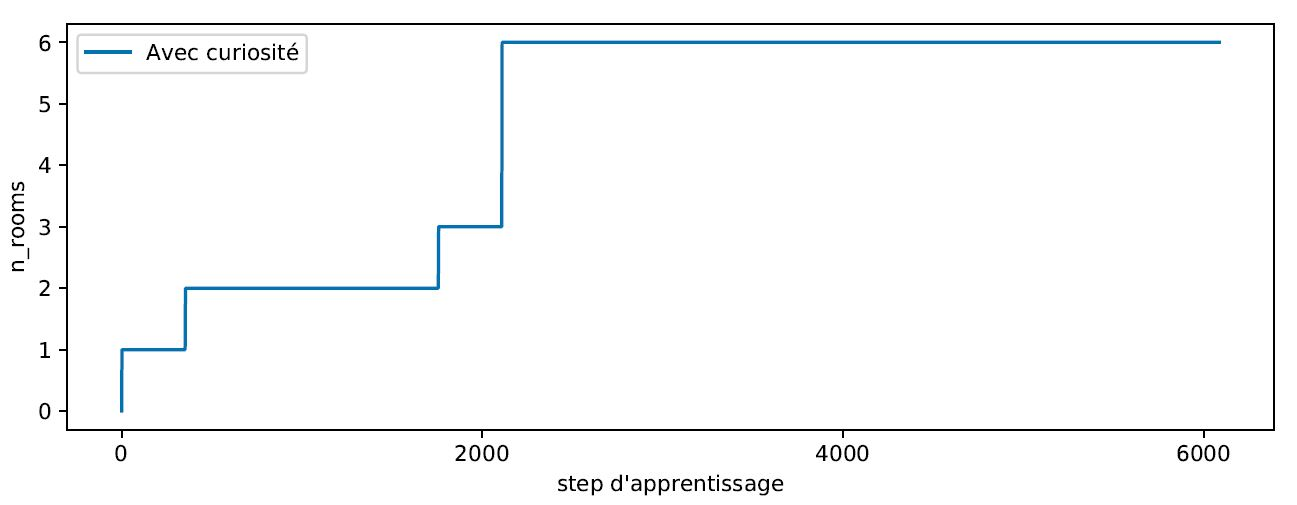
\includegraphics[width=\textwidth]{curiosity_only/curiosity_n_rooms.JPG}
    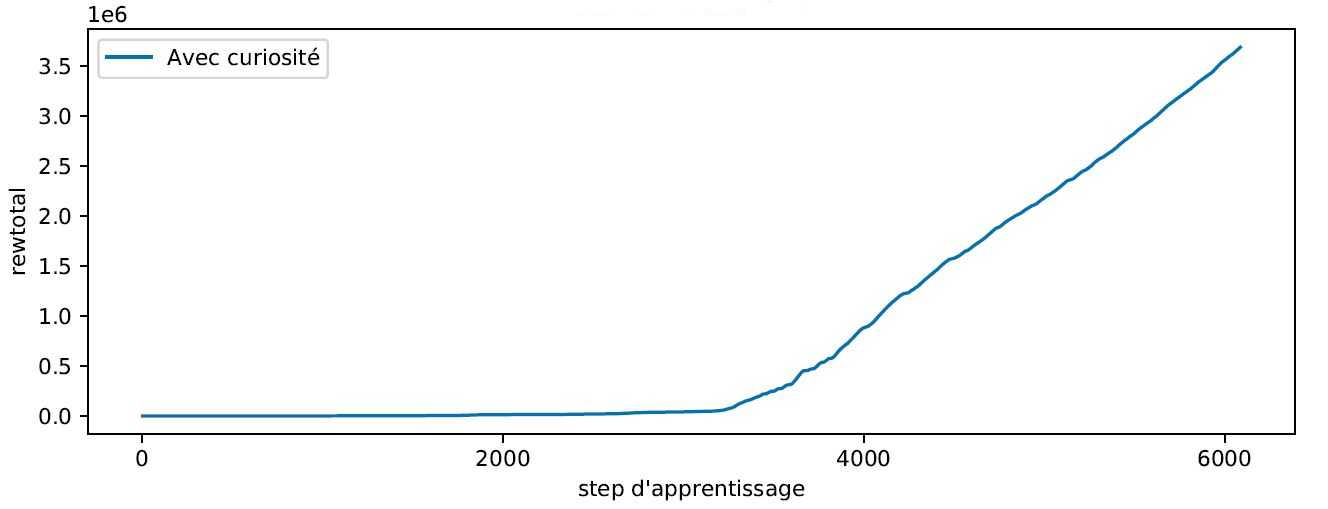
\includegraphics[width=\textwidth]{curiosity_only/curiosity_rewtotal.JPG}
    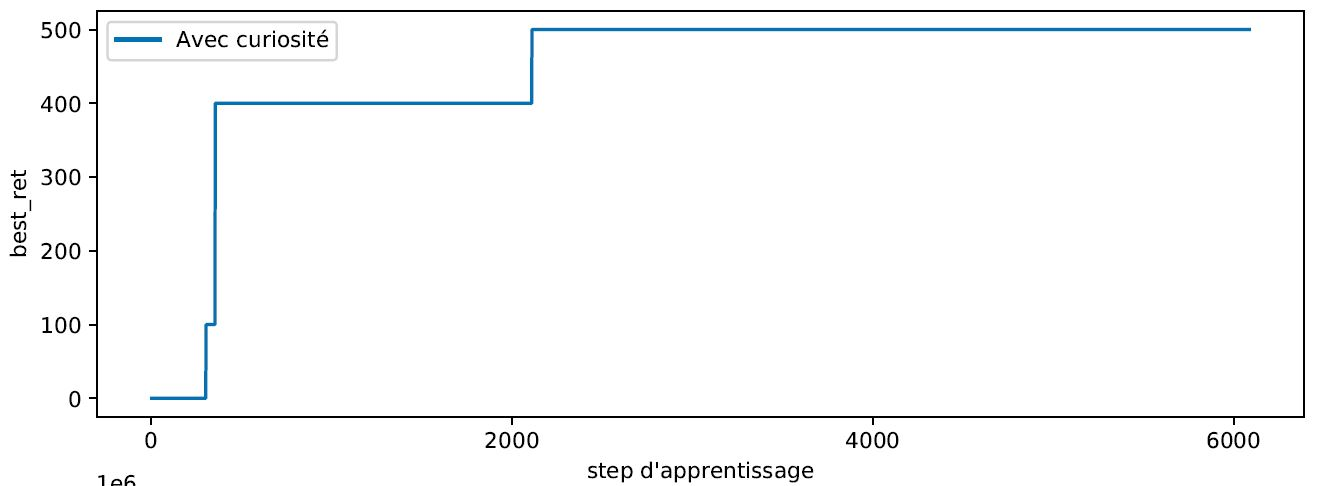
\includegraphics[width=\textwidth]{curiosity_only/curiosity_best_ret.JPG}
    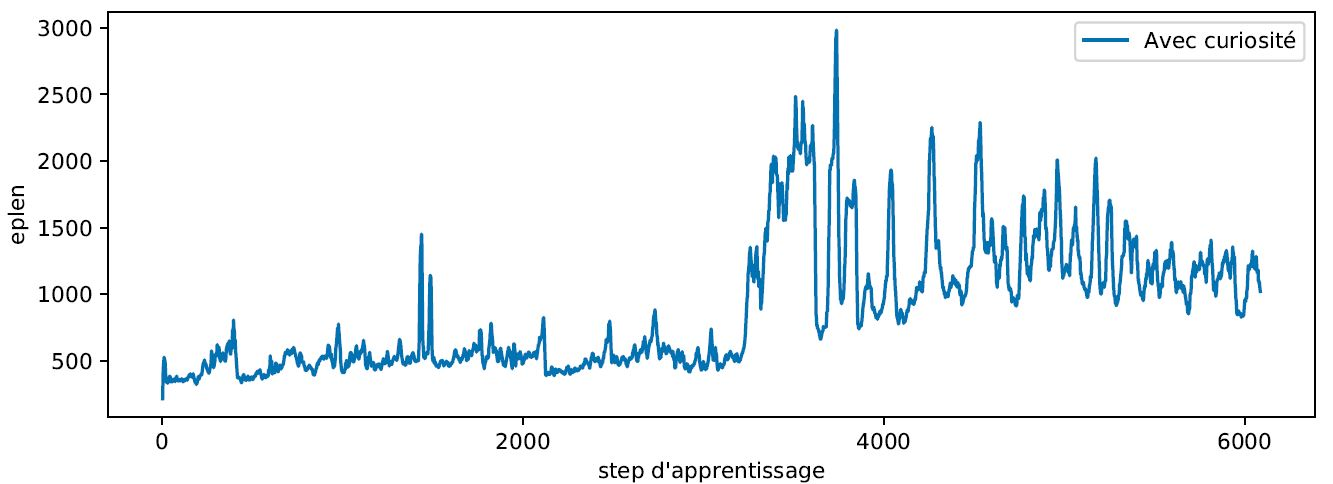
\includegraphics[width=\textwidth]{curiosity_only/curiosity_eplen.JPG}
    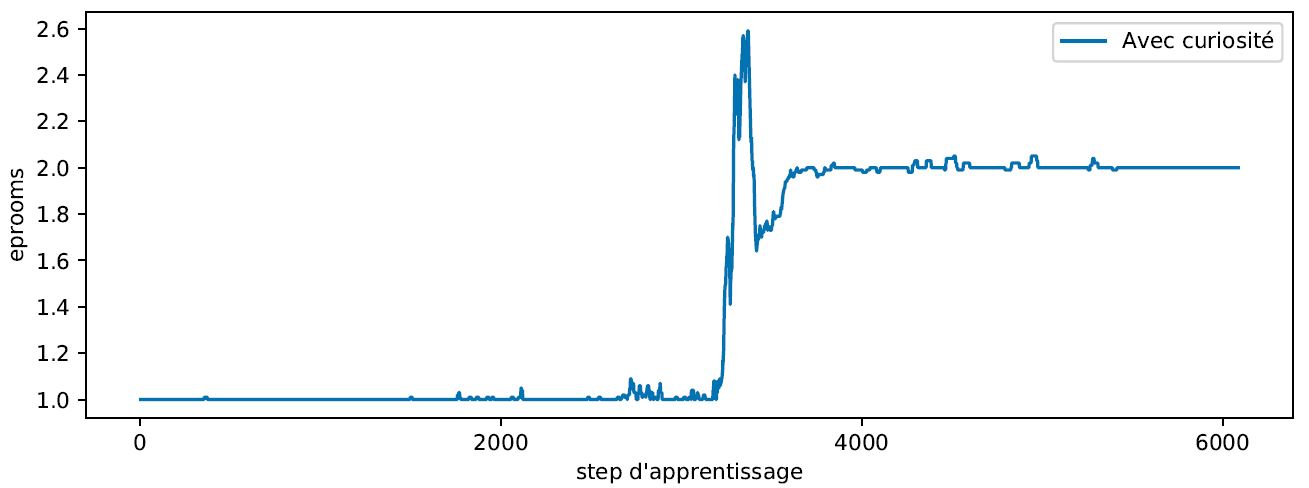
\includegraphics[width=\textwidth]{curiosity_only/curiosity_eprooms.JPG}

\newpage
\subsection*{Annexe 2 - Graphiques d'apprentissage de l'agent avec curiosité et de l'agent avec imitation}
\addcontentsline{toc}{subsection}{Annexe 2}
\label{annexe_2}
    \centering
    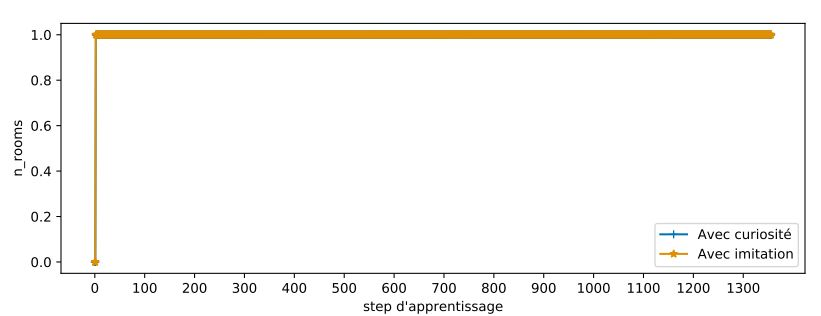
\includegraphics[width=\textwidth]{curiosity_imitation/curiosity_imitation_n_rooms.JPG}
    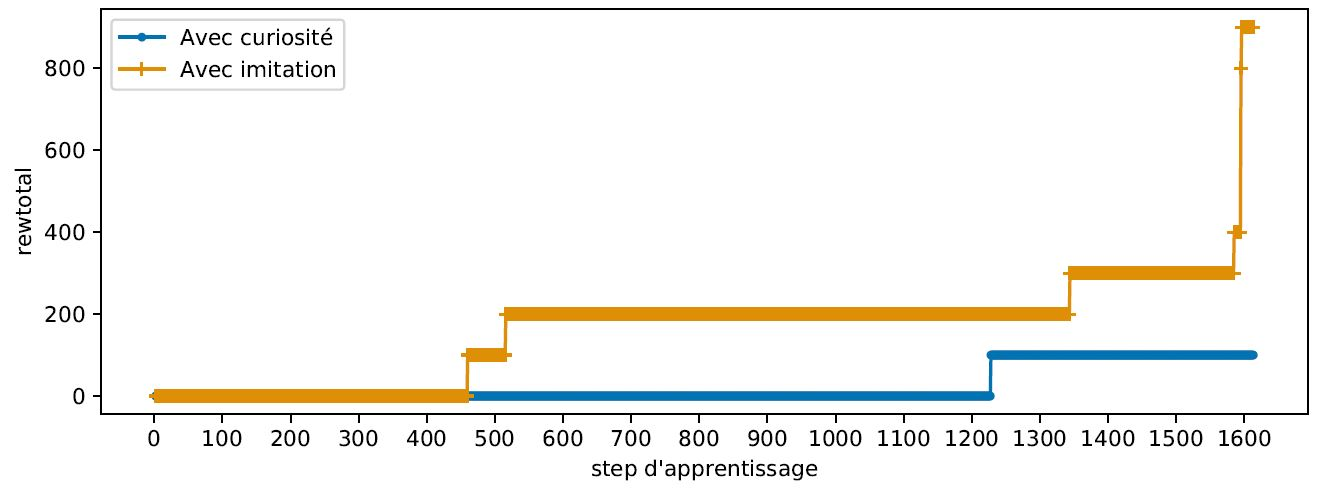
\includegraphics[width=\textwidth]{curiosity_imitation/curiosity_imitation_rewtotal.JPG}
    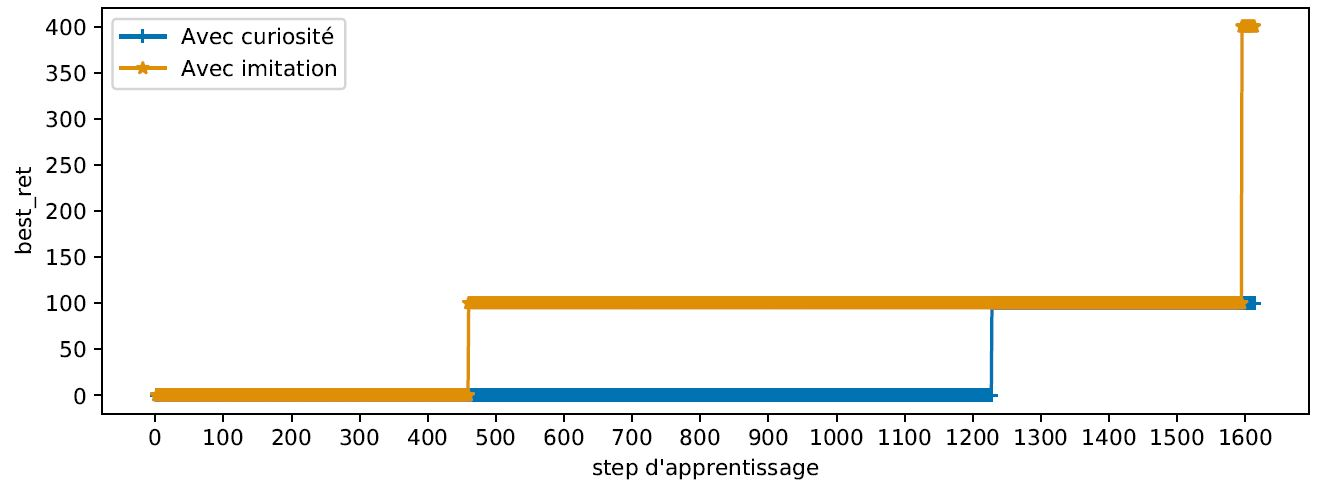
\includegraphics[width=\textwidth]{curiosity_imitation/curiosity_imitation_best_ret.JPG}
    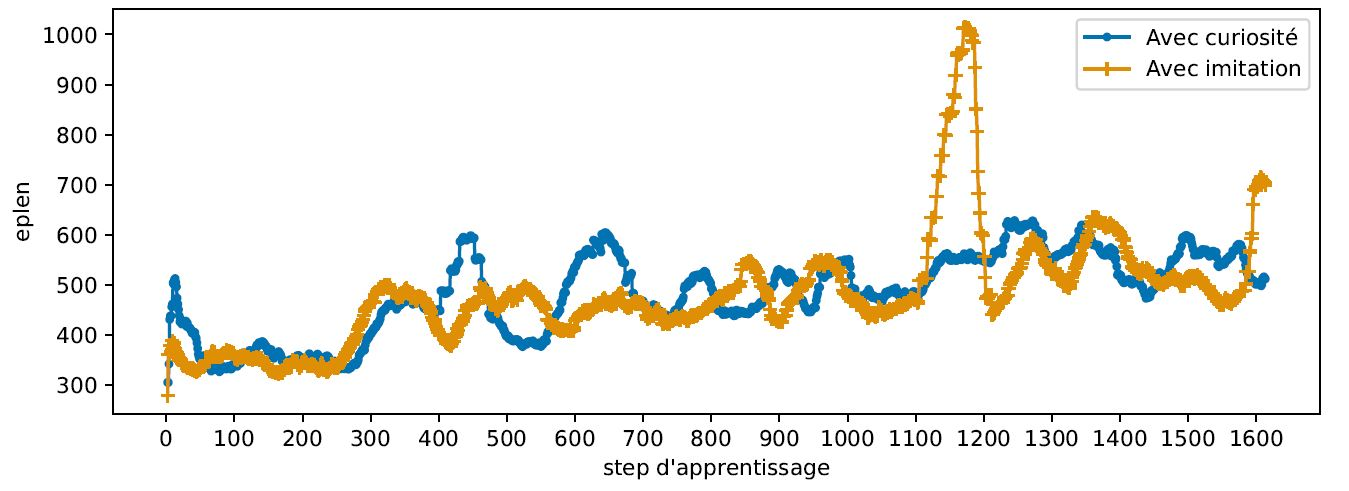
\includegraphics[width=\textwidth]{curiosity_imitation/curiosity_imitation_eplen.JPG}
    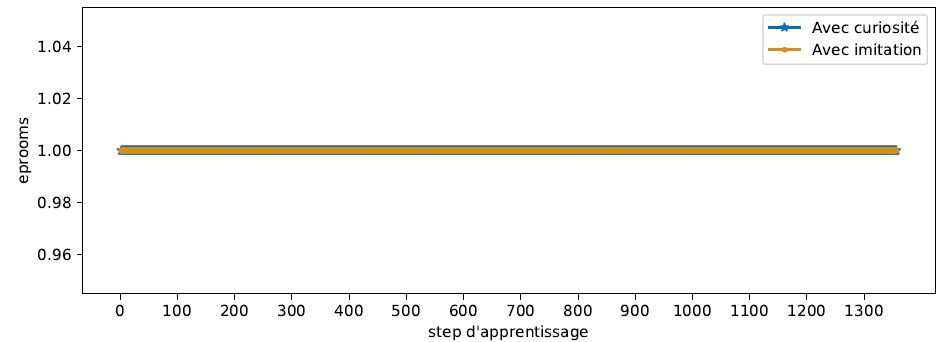
\includegraphics[width=\textwidth]{curiosity_imitation/curiosity_imitation_eprooms.JPG}

\begin{thebibliography}{9}
\addcontentsline{toc}{section}{Bibliographie}
    \bibitem{curiosity}
	  Deepak Pathak, Pulkit Agrawal, Alexei A. Efros, Trevor Darrell,\\
	  \textit{Curiosity-driven Exploration by Self-supervised Prediction},\\
	  Mai 2017,\\
	  \url{https://arxiv.org/abs/1705.05363}

    \bibitem{distillation}
	 Yuri Burda, Harrison Edwards, Amos Storkey, Oleg Klimov,\\
	  \textit{Exploration by Random Network Distillation},\\
	  Octobre 2016,\\
	  \url{https://arxiv.org/abs/1810.12894}

    \bibitem{ngu}
	 Adrià Puigdomènech Badia, Pablo Sprechmann, Alex Vitvitskyi, Daniel Guo, Bilal Piot, Steven Kapturowski, Olivier Tieleman, Martín Arjovsky, Alexander Pritzel, Andew Bolt, Charles Blundell,\\
	  \textit{Never Give Up: Learning Directed Exploration Strategies},\\
	  Février 2020,\\
	  \url{https://arxiv.org/abs/2002.06038}

    \bibitem{agent57}
	 Adrià Puigdomènech Badia, Bilal Piot, Steven Kapturowski, Pablo Sprechmann, Alex Vitvitskyi, Daniel Guo, Charles Blundell,\\
	  \textit{Agent57: Outperforming the Atari Human Benchmark},\\
	  Mars 2020,\\
	  \url{https://arxiv.org/abs/2003.13350}

    \bibitem{distillation_github}
	  \textit{Github repo for random network distillation}\\
	  \url{https://github.com/openai/random-network-distillation}

		\bibitem{sqil}
	  Siddharth Reddy, Anca D. Dragan, Sergey Levine,\\
	  \textit{SQIL: Imitation Learning via Reinforcement Learning with Sparse Rewards},\\
	  Septembre 2019,\\
	  \url{https://arxiv.org/abs/1905.11108}

	\bibitem{montezuma}
	Jeu vidéo \textit{Montezuma's revenge}\\
	\url{https://en.wikipedia.org/wiki/Montezuma%27s_Revenge_(video_game)}
\end{thebibliography}

\end{document}
